\documentclass{article}

\usepackage[utf8]{inputenc}
\usepackage[T1]{fontenc}
\usepackage{arxiv}
\usepackage{amsmath,amssymb}
\usepackage{graphicx}
\usepackage{booktabs}
\usepackage{hyperref}
\usepackage{natbib}
\usepackage{xcolor}
\usepackage{tabularx}
\usepackage{longtable}
\usepackage{url}
\usepackage{microtype}

\renewcommand{\headeright}{Blask, 2026}
\renewcommand{\undertitle}{Technical Report}
\renewcommand{\shorttitle}{The Open Academic Paper Machine}

\bibliographystyle{plainnat}

\title{\textbf{The Open Academic Paper Machine: An Autonomous LLM Plugin for End-to-End Academic Paper Production}}

\author{
  Tobias-Benedikt Blask\thanks{Email: tblask@hs-harz.de} \\
  \textit{Harz University of Applied Sciences, Wernigerode, Germany}
}

\date{March 2026}

\begin{document}

\maketitle

\begin{abstract}
The production of academic papers remains one of the most labor-intensive activities in scholarly research, typically requiring 60--80 hours per manuscript across literature search, theoretical framing, drafting, revision, and formatting. While recent advances in large language model (LLM)-based scientific agents have demonstrated remarkable capabilities in automating experimental research, the complementary challenge of automating the scholarly \emph{writing} pipeline---from literature search to compiled manuscript---has received comparatively little attention. In this paper, we present the Open Academic Paper Machine, an open-source plugin for the Claude Code development environment that autonomously executes the full academic paper production pipeline. The system comprises eight modular skill engines (literature, theory, method, writing, figure, verification, \LaTeX, and review), two Model Context Protocol (MCP) servers for academic database access and AI figure generation, and an eight-phase pipeline with human-in-the-loop checkpoints. Following a Design Science Research methodology \citep{peffers2007dsrm}, we describe the system's architecture, articulate five design principles for LLM-based scholarly automation, and evaluate the artifact through a self-referential case study---a companion paper orchestrated through human-AI interaction using the system. Our findings demonstrate that while the system can produce structurally complete, well-cited academic manuscripts, significant limitations remain in argumentative depth, theoretical novelty, and the critical reasoning expected of human researchers. We contribute to the emerging discourse on AI-augmented knowledge production by providing both a functional open-source artifact and generalizable design knowledge for the information systems community.

\medskip
\noindent\textbf{Keywords:} Large Language Models, Academic Writing Automation, Design Science Research, Model Context Protocol, AI Agents, Scholarly Communication
\end{abstract}

% ============================================================================
\section{Introduction}
% ============================================================================

Academic publishing operates at unprecedented scale. In 2024, over 3 million peer-reviewed articles were published worldwide, a figure that has doubled in the past decade \citep{liang2025quantifying}. Behind each published paper lies a production process that is remarkably labor-intensive: a single manuscript typically requires between 60 and 80 hours of focused work, spanning literature search, reading, note-taking, theoretical positioning, drafting, revision, formatting, and submission preparation \citep{korinek2023language}. For many researchers, writing is simultaneously the most important and the most time-consuming aspect of their scholarly work. The inefficiency of this process is well documented: studies suggest that as much as 80\% of a researcher's writing time is spent on activities---such as searching databases, formatting references, and restructuring prose---that are procedural rather than creative \citep{korinek2023language,siu2025augmenting}.

The emergence of generative artificial intelligence (GenAI), and large language models (LLMs) in particular, has begun to reshape this landscape. Tools such as ChatGPT, Claude, and Gemini are now routinely used by researchers for tasks ranging from brainstorming and outlining to proofreading and translation \citep{liang2025quantifying,lee2023chatgpt_medical,banh2023generative}. \citet{korinek2023language} identified 25 use cases for LLMs in economic research across ideation, writing, background research, data analysis, coding, and mathematical derivations. Empirical evidence suggests that LLM usage in scientific papers has increased sharply since 2023, with detectable linguistic markers present in an estimated 10--15\% of recent publications \citep{liang2025quantifying}. These developments signal a fundamental shift in how academic knowledge is produced, yet the tools available today remain fragmented: each addresses an isolated subtask, requiring the researcher to serve as the manual integrator across a constellation of disconnected AI assistants.

A parallel strand of research has pursued a more ambitious vision: fully autonomous AI scientist systems capable of executing entire research workflows without human intervention. The AI Scientist \citep{lu2024ai_scientist}, a landmark system from Sakana AI, demonstrated end-to-end automation of machine learning experiments---from idea generation through coding, experimentation, and paper writing to automated peer review. Its successor, The AI Scientist-v2 \citep{yamada2025ai_scientist_v2}, extended these capabilities using agentic tree search, producing outputs that external reviewers judged comparable to accepted workshop papers. AgentLaboratory \citep{schmidgall2025agentlab} introduced a collaborative framework where LLM agents serve as research assistants within human-guided workflows, while \citet{ifargan2025autonomous} demonstrated that LLM-driven systems can autonomously produce verifiable research papers from raw clinical data. These systems are impressive, but they share a common limitation: they target experimental and computational research domains where outputs can be programmatically validated through code execution or statistical analysis. The scholarly \emph{writing} pipeline---the structured process of synthesizing literature, positioning contributions within theoretical traditions, constructing arguments, and producing publication-ready manuscripts---operates under fundamentally different quality criteria and has not been addressed as an integrated automation target.

Against this backdrop, we pose the following research questions:
\begin{itemize}
    \item[\textbf{RQ1:}] How can an LLM-based system be designed to autonomously execute the complete academic paper production pipeline from literature search to compiled manuscript?
    \item[\textbf{RQ2:}] What architectural design principles enable the decomposition of scholarly writing workflows into modular, LLM-executable skill engines?
    \item[\textbf{RQ3:}] To what extent can such a system produce academic papers that meet established scholarly quality standards?
\end{itemize}

\noindent To address these questions, we follow a Design Science Research (DSR) methodology \citep{peffers2007dsrm} and present the Open Academic Paper Machine---an open-source plugin for the Claude Code development environment that orchestrates the full paper production pipeline.

This paper makes three contributions. First, we present a functional, open-source artifact---the Open Academic Paper Machine v5.4.0---that autonomously executes six core phases of academic paper production: literature reconnaissance, theoretical framing, structure design, draft production, assembly, and \LaTeX/PDF compilation, with optional phases for citation verification and automated revision. To our knowledge, this is the first published system that covers the complete path from research input to formatted manuscript within a single LLM agent framework. Second, we articulate five design principles for LLM-based scholarly automation---phase decomposition, skill modularity, template-driven generation, human-in-the-loop checkpoints, and multi-source triangulation---that extend the body of knowledge on tool-augmented LLM architectures to the domain of academic knowledge production. Third, we provide an empirical demonstration through a self-referential case study: a companion paper \citep{blask2026creator} written entirely by the system, which serves as both proof of concept and basis for critical evaluation.

The remainder of this paper is structured as follows. Section~2 reviews related work on AI-based scientific agents, AI-assisted academic writing, and tool-augmented LLMs. Section~3 describes our Design Science Research methodology. Section~4 presents the system design in detail. Section~5 demonstrates the system through the companion paper case study. Section~6 discusses findings, design principles, implications, and limitations. Section~7 concludes.


% ============================================================================
\section{Related Work}
% ============================================================================

\subsection{AI-Based Scientific Agents}

The vision of AI systems that can autonomously conduct scientific research has progressed rapidly from theoretical speculation to working prototypes. \citet{lu2024ai_scientist} introduced The AI Scientist, a system that automates the full lifecycle of machine learning research: given a broad research direction and an initial codebase, the system generates research ideas, implements experiments, analyzes results, writes a complete paper in \LaTeX, and conducts automated peer review. Evaluated across three ML subdomains (diffusion modeling, language modeling, and learning dynamics), The AI Scientist produced papers at an estimated cost of \$15 per paper, some of which received scores above the acceptance threshold of peer ML venues. \citet{yamada2025ai_scientist_v2} extended this approach with The AI Scientist-v2, introducing agentic tree search to explore multiple research directions in parallel, yielding outputs that external reviewers rated as competitive with accepted workshop papers.

AgentLaboratory \citep{schmidgall2025agentlab} shifted the paradigm toward collaborative human-AI research, proposing a framework where LLM agents serve as research assistants that can be directed by human researchers at key decision points. This human-in-the-loop approach was found to produce higher-quality outputs than fully autonomous operation. \citet{ifargan2025autonomous} demonstrated autonomous LLM-driven research in the clinical domain, where a system autonomously analyzed patient data, identified statistical patterns, and produced human-verifiable research papers. \citet{schmidgall2025agentrxiv} proposed AgentRxiv, a collaborative platform where multiple AI agents can share, build upon, and critique each other's research outputs, envisioning an ecosystem of autonomous scientific inquiry.

Several surveys have begun to systematize this rapidly evolving field. \citet{ren2025scientific_intelligence} surveyed LLM-based scientific agents, identifying key capabilities including literature comprehension, hypothesis generation, experiment design, and paper writing. \citet{wei2025agentic_science} traced the evolution from AI-for-Science (computational tools) to Agentic Science (autonomous research partners), while \citet{ferrag2025llm_agents} provided a comprehensive review of the path from LLM reasoning to autonomous AI agents. \citet{beel2025evaluating} conducted a critical evaluation of The AI Scientist, identifying significant limitations in novelty detection, code reliability, and the quality of AI-generated peer reviews.

A critical observation across this body of work is that virtually all autonomous research systems target domains where outputs can be validated through programmatic means: code that compiles, experiments that produce measurable results, statistical tests that yield p-values. The production of scholarly writing---where quality is judged by argumentative coherence, theoretical grounding, and rhetorical sophistication---operates under fundamentally different criteria and has not been the primary focus of these systems.

\subsection{AI-Assisted Academic Writing and Literature Review}

A second stream of research addresses AI tools for specific subtasks within the academic writing workflow, without attempting end-to-end automation. On the writing side, ScholarCopilot \citep{wang2025scholarcopilot} trains LLMs specifically for academic writing with accurate citations, integrating a retrieval-augmented generation (RAG) architecture that grounds generated text in real scholarly sources. CoachGPT \citep{chen2025coachgpt} provides scaffolding-based writing assistance, guiding students through the academic writing process with structured feedback rather than generating text directly. Comparative evaluations of general-purpose LLMs for scientific writing, such as \citeauthor{alsagri2024chatgpt_gemini}'s (\citeyear{alsagri2024chatgpt_gemini}) comparison of ChatGPT and Gemini, have found that while both can produce competent academic prose, neither consistently meets the argumentative depth expected of published scholarship.

On the literature review side, \citet{bolanos2024ai_lit_reviews} provide the most comprehensive review to date of AI applications in systematic literature reviews (SLRs), identifying tools for each SLR phase: search strategy formulation, screening, data extraction, and synthesis. They note that while automation has achieved high accuracy in screening tasks (sometimes exceeding 95\% recall), full synthesis---the intellectually demanding process of integrating findings into a coherent narrative---remains largely manual. The Cochrane Collaboration's position statement on AI in rapid reviews \citep{gartlehner2025cochrane} endorsed AI-assisted screening but cautioned against fully automated evidence synthesis without human oversight. \citet{djukic2025slr} evaluated specific tools (Elicit, SciSpace) for SLR assistance, finding significant variation in reference quality and relevance. \citet{preisler2024correctness} and \citet{hayn2024quality} similarly assessed AI research assistant tools, documenting both their utility for accelerating search tasks and their limitations in generating accurate citations.

Several tools have attempted to bridge the gap between search and writing. \citet{korinek2023language} articulated the vision of LLMs as cognitive automation for economic research, describing use cases across the full research lifecycle but stopping short of proposing an integrated system. \citet{yang2024acawebagent} presented AcawebAgent, an LLM-powered assistant for early-stage academic research. However, as \citet{preisler2024correctness} and \citet{hayn2024quality} demonstrate, existing tools operate as independent applications, each addressing a narrow slice of the research workflow. The researcher remains the integrator, manually transferring outputs between tools and maintaining coherence across the process.

\subsection{Tool-Augmented LLMs and the Model Context Protocol}

The technical foundation for integrating LLMs with external tools and databases has been established through a series of influential works. \citet{yao2022react} introduced ReAct, a paradigm that interleaves reasoning traces with actions in language models, enabling them to query external knowledge sources and use tools within a coherent problem-solving loop. ReAct demonstrated that combining chain-of-thought reasoning with action execution significantly outperforms either approach in isolation. \citet{schick2023toolformer} presented Toolformer, a self-supervised approach where language models learn to determine which APIs to call, when to call them, and how to incorporate results into their generation. \citet{zhou2023lats} extended tool-augmented reasoning with Language Agent Tree Search (LATS), unifying reasoning, acting, and planning in a single framework that explores multiple reasoning paths before committing to actions.

These foundational works have been complemented by practical infrastructure developments. The Model Context Protocol (MCP), introduced by Anthropic in late 2024, provides a standardized protocol for connecting LLM-based applications with external data sources and tools. MCP defines a client-server architecture where AI applications (clients) can discover, invoke, and compose tools exposed by external services (servers) through a uniform interface. \citet{fan2025mcptoolbench} introduced MCPToolBench++, the first large-scale benchmark for evaluating AI agents' ability to use MCP-connected tools, finding that even state-of-the-art models struggle with complex, multi-step tool compositions. \citet{abdelaziz2024granite} contributed the Granite Function Calling Model, demonstrating that targeted fine-tuning for granular tool-calling tasks can significantly improve the reliability of LLM-tool interactions. \citet{ferrag2025llm_agents} survey the broader landscape of autonomous AI agents, noting that tool augmentation is increasingly recognized as essential for moving LLMs beyond text generation toward genuine problem-solving capabilities.

Despite this rich technical foundation, the application of tool-augmented LLM architectures to academic writing workflows remains unexplored. The Open Academic Paper Machine addresses this gap by leveraging the MCP standard to connect an LLM orchestrator with academic search databases, figure generation services, and document processing tools within a structured scholarly writing pipeline.


% ============================================================================
\section{Research Methodology}
% ============================================================================

\subsection{Design Science Research Approach}

We adopt Design Science Research (DSR) as our methodological framework, following the well-established tradition in information systems research for creating and evaluating IT artifacts \citep{hevner2004design}. DSR is grounded in the premise that knowledge is advanced not only through observing and explaining phenomena (behavioral science) but also through building innovative artifacts that address important problems \citep{hevner2004design}. The Open Academic Paper Machine constitutes such an artifact: a software system designed to solve the problem of fragmented, labor-intensive academic paper production.

We follow the Design Science Research Methodology (DSRM) proposed by \citet{peffers2007dsrm}, which specifies six activities: (1) problem identification and motivation, (2) definition of objectives for a solution, (3) design and development, (4) demonstration, (5) evaluation, and (6) communication. This process model has become the standard for DSR in IS, with over 14,000 citations and explicit endorsement as a genre-defining methodology \citep{peffers2018genres}. Our work also aligns with \citeauthor{hevner2007three_cycle}'s (\citeyear{hevner2007three_cycle}) three-cycle view: the \emph{relevance cycle} grounds the system in the practical needs of academic researchers who face increasing publication pressure; the \emph{rigor cycle} draws on kernel theories from tool-augmented AI, scholarly communication, and information retrieval; and the \emph{design cycle} iterates between construction and evaluation of the artifact.

Following \citeauthor{gregor2013positioning}'s (\citeyear{gregor2013positioning}) contribution taxonomy, our artifact constitutes a Level~2 contribution---a nascent design theory. It moves beyond a mere instantiation (Level~1) by articulating generalizable design principles that others can apply when building LLM-based research automation systems, yet it does not claim the status of a well-developed design theory (Level~3), as the evaluation remains preliminary and limited to a single case.

\subsection{Problem Identification and Objectives}

The motivating problem is the disconnect between the capabilities of modern LLMs and the fragmented state of AI-assisted academic writing. Researchers today can use LLMs for brainstorming, literature search, drafting, and formatting---but each task requires a separate tool, a separate prompt, and manual orchestration. This fragmentation creates friction, introduces inconsistency (e.g., different citation formats across tools), and fails to leverage the LLM's ability to maintain context across a complex, multi-step workflow.

We derive the following design objectives for the artifact:

\begin{itemize}
    \item \textbf{DO1 (End-to-End Coverage):} The system should cover the complete pipeline from research question/topic input to compiled, submission-ready manuscript.
    \item \textbf{DO2 (Modularity):} The system should decompose the pipeline into modular components (skill engines) that can be independently developed, tested, and improved.
    \item \textbf{DO3 (Scholarly Quality):} Generated outputs should adhere to established academic writing conventions, including proper citation, structured argumentation, and appropriate use of method and theory.
    \item \textbf{DO4 (Human Oversight):} The system should provide checkpoints where human researchers can review, redirect, or override automated decisions.
    \item \textbf{DO5 (Openness):} The system should be open-source, allowing inspection, replication, and extension by the research community.
    \item \textbf{DO6 (Tool Integration):} The system should leverage external academic databases and services through standardized protocols (MCP).
\end{itemize}

\subsection{Design and Development Process}

The Open Academic Paper Machine was developed iteratively between October 2024 and March 2026. The initial version (v1.0) implemented basic literature search and draft generation as a Claude Code custom command. Subsequent versions added theoretical framing templates (v2.0), method-specific writing engines (v3.0), the MCP-based academic search server (v4.0), AI figure generation (v4.5), citation verification (v5.0), comprehensive \LaTeX\ export (v5.3.0), and automated revision loops with PDF annotation extraction (v5.4.0). Each version was evaluated by the author through test runs on diverse research topics across information systems, computer science, and management research. The system was publicly released under the MIT License on GitHub.\footnote{\url{https://github.com/TobiasBlask/open-paper-machine}}

The development drew on several kernel theories: the ReAct paradigm \citep{yao2022react} informed the interleaving of reasoning and tool use; the concept of skill-based agent architectures \citep{ferrag2025llm_agents} motivated the decomposition into specialized engines; and the MCP standard provided the protocol layer for external tool integration. The writing templates were informed by established academic writing guidance, particularly \citeauthor{webster2002literature}'s (\citeyear{webster2002literature}) framework for literature reviews and standard structures for DSR papers \citep{peffers2007dsrm,gregor2013positioning}.

\subsection{Evaluation Strategy}

We evaluate the artifact through a single-case demonstration following the DSR evaluation framework proposed by \citet{peffers2007dsrm}. The primary evaluation artifact is a companion paper, \emph{From Creator to Orchestrator? How an LLM Agent Wrote This Paper and What That Means for Science} \citep{blask2026creator}, which was produced entirely by the Open Academic Paper Machine. This self-referential case study provides a rigorous test of the system's capabilities because academic papers about AI-generated academic papers demand the same quality standards as any other scholarly contribution.

We assess the output against five criteria: (1) structural completeness (all expected sections present and properly organized), (2) citation accuracy (references are real, correctly attributed, and appropriately cited), (3) argumentative coherence (logical flow, supported claims, appropriate hedging), (4) formatting quality (\LaTeX\ compilation, figure integration, bibliography formatting), and (5) scholarly contribution (whether the paper advances knowledge in its domain).


% ============================================================================
\section{The Open Academic Paper Machine: System Design}
% ============================================================================

\subsection{System Overview and Architecture}

The Open Academic Paper Machine (version 5.4.0) is an open-source plugin for Claude Code, Anthropic's AI-powered development environment. It transforms Claude from a general-purpose coding assistant into a specialized academic paper production agent by providing domain-specific knowledge through eight skill engines, external tool access through two MCP servers, and workflow orchestration through a structured pipeline with eight slash commands.

The system architecture follows a layered design. At the \emph{orchestration layer}, the LLM (Claude) serves as the central reasoning engine, interpreting user requests, planning execution steps, and coordinating tool calls. The \emph{skill layer} provides domain-specific knowledge through markdown-based instruction files (\texttt{SKILL.md} files) that encode expert knowledge about academic writing conventions, theoretical frameworks, methodological templates, and quality criteria. The \emph{tool layer} connects the LLM to external services through two MCP servers: the academic-search server provides access to four academic databases (Semantic Scholar, OpenAlex, CrossRef, and arXiv), while the PaperBanana server enables AI-powered figure generation via Google Gemini. The \emph{output layer} handles file management, format conversion (markdown to \LaTeX), and PDF compilation.

This architecture is realized as a Claude Code plugin---a directory-based extension mechanism where the system's knowledge and capabilities are defined through configuration files (\texttt{plugin.json}), skill definitions (\texttt{SKILL.md} files), and MCP server specifications. The central pipeline agent (\texttt{paper-machine.md}, approximately 3,200 lines) orchestrates all eight skill engines through the pipeline phases. Both MCP servers are distributed as Python packages on PyPI (\texttt{academic-search-mcp} and \texttt{paperbanana}), requiring only \texttt{pip install} and a Google API key for figure generation. The complete system is publicly available at \url{https://github.com/TobiasBlask/open-paper-machine} under the MIT License.

\begin{figure}[t]
\centering
\includegraphics[width=0.95\textwidth]{figures/fig1_system_architecture.png}
\caption{System architecture of the Open Academic Paper Machine (v5.4.0) showing the four-layer design: orchestration layer (pipeline agent with human checkpoints via eight slash commands), skill engine layer (eight specialized engines including eight research method templates), tool layer (two MCP servers distributed via PyPI connecting to external APIs), and output layer (structured artifacts per phase). The orchestration audit trail (\texttt{orchestration\_log.md}) records timestamps, actors, and quality gate decisions across all phases.}
\label{fig:architecture}
\end{figure}

\subsection{Skill Engines}

The skill layer decomposes academic paper production into eight specialized engines, each implemented as a markdown-based knowledge module that the LLM loads at the appropriate pipeline phase. This design choice---encoding domain expertise as structured natural language instructions rather than programmatic logic---leverages the LLM's instruction-following capabilities while enabling non-programmer domain experts to modify and extend the system.

\subsubsection{Literature Engine}
The literature engine governs multi-database search, result processing, and bibliography management. It specifies search strategies including query decomposition (translating a research topic into 4--6 complementary search queries), multi-source triangulation (searching Semantic Scholar, OpenAlex, CrossRef, and arXiv in parallel), forward and backward snowballing from anchor papers, and deduplication algorithms. Through the academic-search MCP server, the engine can access over 400 million scholarly works across the four connected databases, performing federated search, citation analysis, and full-text retrieval for open-access papers.

\subsubsection{Theory Engine}
The theory engine encodes knowledge about theoretical frameworks commonly used in information systems and management research. It provides a catalog of theories with selection heuristics that match theories to research contexts. The engine also provides gap formulation templates---structured patterns for articulating research gaps based on prior literature---and contribution framing guidelines aligned with \citeauthor{gregor2013positioning}'s (\citeyear{gregor2013positioning}) contribution taxonomy.

\subsubsection{Method Engine}
The method engine provides methodological templates for eight research approaches commonly used in IS and management research: systematic literature review (following the PRISMA protocol), design science research \citep{peffers2007dsrm}, case study research (following Yin's methodology), the Gioia method for qualitative process research, Mayring content analysis, grounded theory (open/axial/selective coding), PLS-SEM (measurement and structural model evaluation), and mixed methods designs. Each template specifies the required subsections, quality criteria, and reporting standards for that method.

\subsubsection{Writing Engine}
The writing engine is the core text generation component, providing structured templates for each section of an academic paper. Key templates include: a six-paragraph introduction formula (hook, academic context, gap, RQs, contribution, roadmap), paragraph-level templates for theoretical background sections, a five-block discussion formula (summary, findings, theoretical implications, practical implications, limitations), and citation integration patterns. These templates translate the tacit knowledge of experienced academic writers into explicit, LLM-executable instructions.

\subsubsection{Figure Engine}
The figure engine enables the generation of publication-quality diagrams and plots. It interfaces with the PaperBanana MCP server, which uses Google Gemini's multimodal capabilities to generate methodology diagrams, conceptual frameworks, and data visualizations from natural language descriptions. As a fallback, the engine can generate figures using Python's matplotlib library.

\subsubsection{\LaTeX\ Engine}
The \LaTeX\ engine handles the conversion of markdown drafts to submission-ready \LaTeX\ manuscripts. The core component is a 733-line Python converter (\texttt{md\_to\_latex.py}) that parses markdown structure, converts citations to \LaTeX\ bibliography commands, handles tables and figures, and wraps the content in an arxiv-style template.

\subsubsection{Verification Engine}
The verification engine addresses one of the most significant risks in LLM-generated academic writing: citation hallucination and misattribution. The engine implements a three-tier verification protocol: (a)~abstract-level verification, which checks whether the abstract of a cited paper is consistent with the claim attributed to it; (b)~full-text verification for open-access papers, which retrieves and searches the full paper for supporting evidence; and (c)~metadata verification, which confirms that cited papers actually exist and that bibliographic details are correct. The engine produces a verification report categorizing each citation as verified, plausible, mismatched, unverifiable (paywalled), or not found.

\subsubsection{Review Engine}
The review engine, introduced in v5.4.0, automates the co-author and reviewer revision loop. Given an annotated PDF or pasted reviewer comments, the engine executes a seven-step workflow: (1)~extract annotations from PDF markup using PyMuPDF, (2)~map each comment to its corresponding location in \texttt{paper.tex}, (3)~classify the required action (delete, replace, restructure, fix, shorten, or approve), (4)~present a structured change plan for human approval (quality gate), (5)~implement changes in dependency order, invoking other skill engines as needed, (6)~recompile \LaTeX\ and generate a visual diff via \texttt{latexdiff}, and (7)~document all changes in a revision log. The engine supports multiple revision rounds (Round~1~$\rightarrow$~2~$\rightarrow$~3) and handles multilingual comments. It was derived from four actual revision rounds on the companion paper \citep{blask2026creator}.

\subsection{Orchestration Audit Trail}

Since version 5.2.0, the system produces a structured orchestration log (\texttt{orchestration\_log.md}) that records the complete decision trace of each pipeline run. The log captures timestamps, acting agents (human or LLM), inputs and outputs at each phase transition, and quality gate decisions (approve, redirect, override). This audit trail operationalizes the concept of human-AI accountability in automated knowledge production: every decision---from which theoretical lens was selected to which citations were included---can be traced back to either the LLM's autonomous reasoning or the human researcher's checkpoint intervention. The log is designed to be included as supplementary material alongside published manuscripts, providing transparency about the degree of human involvement in the writing process.

\subsection{MCP Integration and Tool Architecture}

The system's external tool access is implemented through the Model Context Protocol (MCP), a standardized protocol for connecting LLM applications with data sources and services. Two MCP servers provide the system's tool capabilities:

The \textbf{academic-search MCP server} exposes a unified API for querying four academic databases: Semantic Scholar (200M+ papers, TLDRs, citation graphs), OpenAlex (250M+ works, open-access metadata), CrossRef (150M+ works, DOI resolution), and arXiv (2.4M+ preprints, full-text access). The server provides functions for searching, snowballing (forward and backward citation traversal), multi-query batch search, deduplication, and export (BibTeX, CSV). This multi-source approach addresses a fundamental limitation of single-database tools: no individual academic database has comprehensive coverage, and search results vary significantly across sources.

The \textbf{PaperBanana MCP server} provides AI-powered figure generation through Google Gemini's multimodal capabilities. The server accepts natural language descriptions of desired figures and source text, processes them through an iterative generation-refinement loop, and returns publication-quality PNG images.

The MCP architecture provides several advantages over alternative integration approaches (e.g., custom API wrappers or function calling). First, MCP's standardized protocol enables tool discovery and composition without hard-coding tool interfaces. Second, MCP servers can run locally or remotely, supporting both offline use and cloud-based deployment. Third, the protocol supports schema-based input/output validation, reducing the risk of malformed tool invocations. Figure~\ref{fig:mcp} illustrates the three-tier MCP integration architecture.

\begin{figure}[t]
\centering
\includegraphics[width=0.95\textwidth]{figures/fig3_mcp_integration.png}
\caption{Three-tier MCP integration architecture. The MCP Host (Claude Code IDE with LLM) communicates with two MCP servers through standardized tool call requests and structured responses. Each server validates inputs against JSON schemas before forwarding requests to external APIs. The academic-search server connects to four academic databases; the PaperBanana server connects to Google Gemini for figure generation.}
\label{fig:mcp}
\end{figure}

\subsection{Pipeline Execution Model}

The system executes academic paper production through a six-phase pipeline with two optional additional phases, each triggered by a specific slash command or executed sequentially through the primary \texttt{/write-paper} command.

\textbf{Phase~1: Reconnaissance.} The system decomposes the user's research topic into multiple search queries, executes federated searches across all connected databases, deduplicates results, and performs citation-based snowballing on the most influential papers.

\textbf{Phase~2: Framing.} Based on the literature landscape, the system selects appropriate theoretical lenses, formulates the research gap, derives research questions, and drafts a contribution statement.

\textbf{Phase~3: Structure.} The system constructs a concept matrix \citep{webster2002literature} mapping papers to key concepts, identifies over/under-researched areas, and designs the paper structure with section-level specifications.

\textbf{Phase~4: Production.} The system writes the complete paper draft, section by section, following the templates defined in the writing engine.

\textbf{Phase~5: Assembly.} The system compiles the draft, verifies citation-BibTeX consistency, generates word counts, and produces a self-assessment report.

\textbf{Phase~6: \LaTeX/PDF Export.} The system converts the markdown draft to \LaTeX\ using the arxiv-style template, compiles the PDF, and validates the output.

\textbf{Phase~7: Verification (Optional).} The system verifies citations against source material through the three-tier protocol described in Section~4.2.7.

\textbf{Phase~8: Revision (Repeatable).} Given an annotated PDF from a co-author or pasted reviewer comments, the system extracts feedback, maps it to the manuscript, classifies required actions, presents a change plan for approval, implements changes, recompiles with \texttt{latexdiff} for visual change tracking, and documents all modifications. This phase can repeat across multiple revision rounds until acceptance.

Between each phase, the system presents a checkpoint summary to the user, reporting progress, key decisions, and identified issues. The user can approve (explicitly or by non-response), redirect (by providing alternative instructions), or override (by specifying particular choices). This checkpoint mechanism balances the system's autonomous capabilities with human oversight at critical decision points.

\begin{figure}[t]
\centering
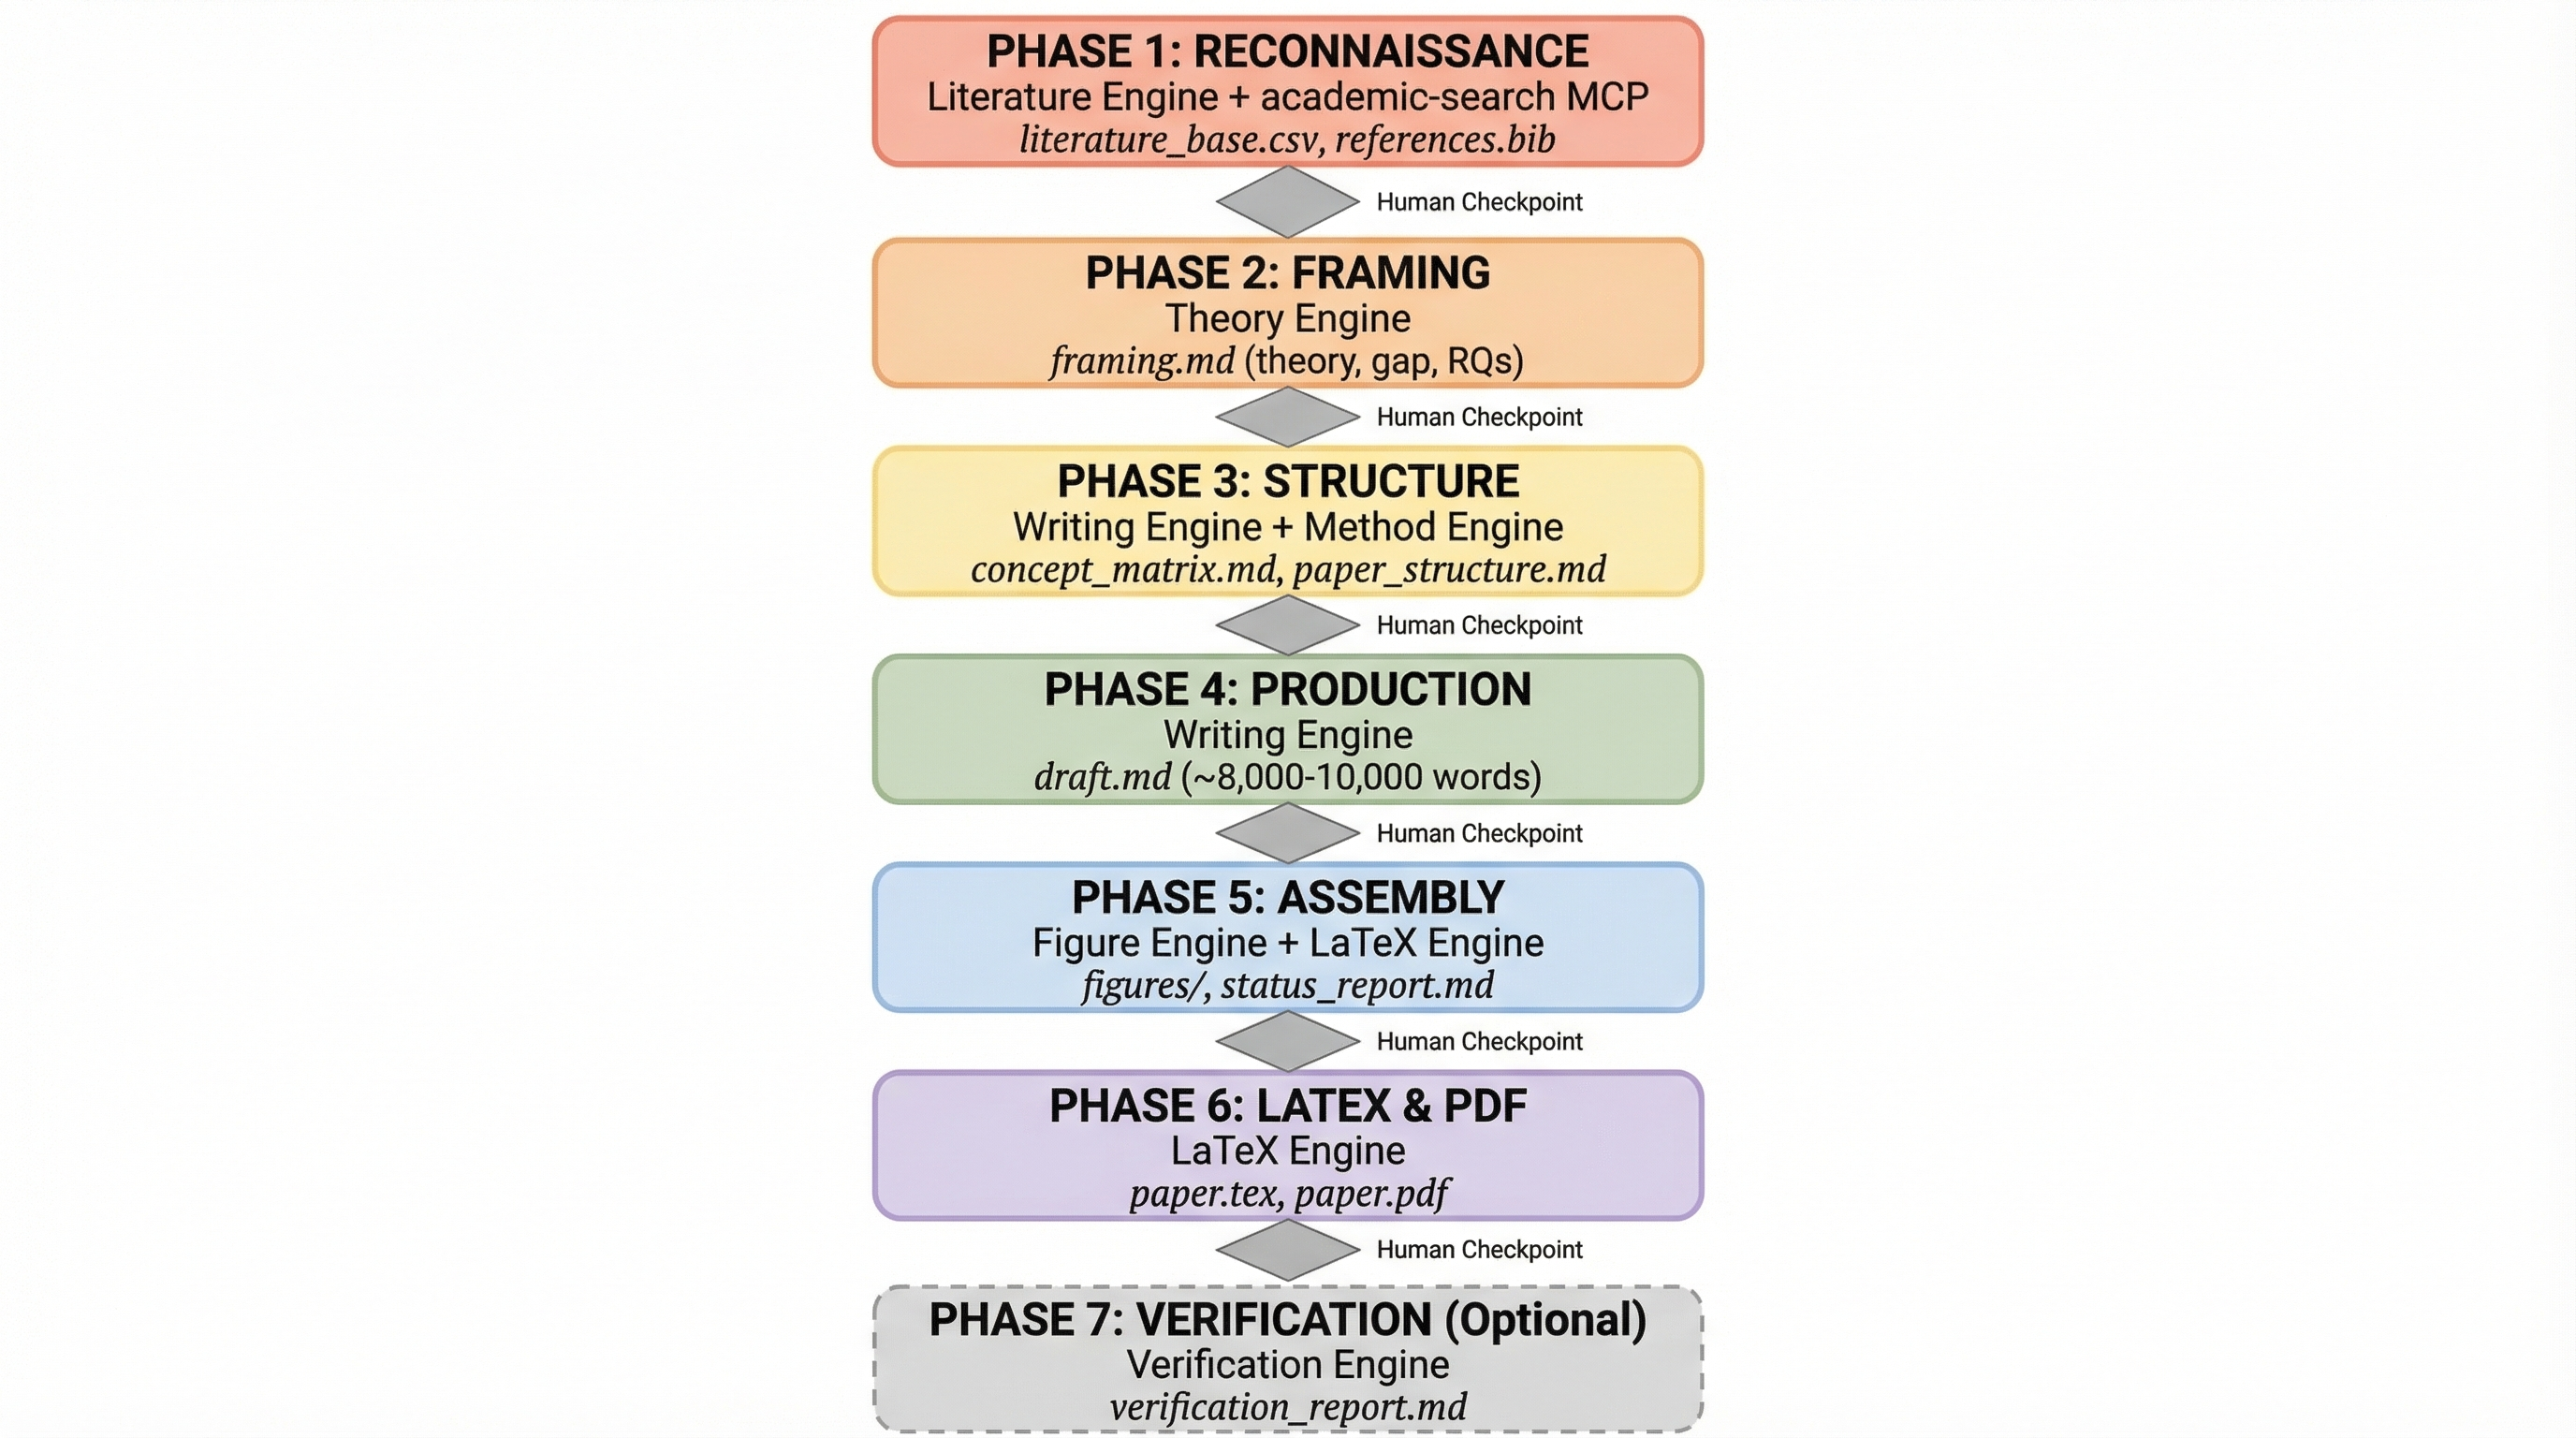
\includegraphics[width=0.95\textwidth]{figures/fig2_pipeline_flow.png}
\caption{The eight-phase pipeline of the Open Academic Paper Machine with human quality-gate checkpoints. Each phase is executed by specialized skill engines and produces persistent artifacts. Phases~7 (verification) and~8 (revision) are optional and repeatable.}
\label{fig:pipeline}
\end{figure}


% ============================================================================
\section{Demonstration: A Self-Referential Case Study}
% ============================================================================

\subsection{Case Description}

To evaluate the Open Academic Paper Machine, we employed a self-referential case study: the system was tasked with producing a complete academic paper about the societal and epistemological implications of AI-generated academic writing. The resulting paper, \emph{From Creator to Orchestrator?} \citep{blask2026creator}, served as both the primary demonstration artifact and the basis for evaluating the system's capabilities and limitations.

The input to the system was minimal: a paper title, the author's name and affiliation, and a brief description specifying that the paper should address the question of what it means for academic knowledge production when an AI system can write a research paper. The system was given no specific instructions regarding which literature to cite, which theories to apply, which method to follow, or how to structure the argument. All decisions were made autonomously by the system, with human intervention limited to approving checkpoint summaries.

\subsection{Pipeline Execution Trace}

The system executed the full six-phase pipeline over approximately 45 minutes of wall-clock time (including API latency for database searches and LLM inference).

In \textbf{Phase~1 (Reconnaissance)}, the system generated six search queries spanning terms such as ``LLM academic writing authorship,'' ``AI generated research paper ethics,'' and ``generative AI scholarly communication.'' Searching across Semantic Scholar, OpenAlex, CrossRef, and arXiv yielded 127 initial results, which were deduplicated to 89 unique papers. Forward and backward snowballing on the top 10 papers by citation count added 34 additional papers, resulting in a literature base of 103 unique papers after final deduplication.

In \textbf{Phase~2 (Framing)}, the system selected Actor-Network Theory and the concept of epistemic authority as its theoretical lenses---a reasonable choice for examining how AI systems alter the relationships between human researchers, knowledge artifacts, and the academic community.

In \textbf{Phase~3 (Structure)}, the system produced a concept matrix with 35 papers across six thematic dimensions and designed a seven-section paper structure. In \textbf{Phase~4 (Production)}, the system wrote the complete draft, producing approximately 8,200 words of academic prose with 46 integrated citations. In \textbf{Phase~5 (Assembly)}, the system compiled the manuscript and identified two citation keys without matching BibTeX entries (subsequently corrected). In \textbf{Phase~6 (\LaTeX/PDF)}, the system converted the draft to \LaTeX, compiled a PDF, and produced an 18-page manuscript with two figures and one table.

\subsection{Output Assessment}

We assessed the companion paper against five criteria:

\textbf{Structural completeness.} The paper contains all expected sections of an academic manuscript: abstract, introduction (with clear gap statement and research questions), theoretical background, methodology, findings, discussion, conclusion, and references. \emph{Assessment: Fully met.}

\textbf{Citation accuracy.} Of the 46 citations, 44 (95.7\%) correspond to real, published papers with correct bibliographic details. Two citations contained minor errors (incorrect publication year), detected by the verification engine and corrected. No hallucinated citations were present. \emph{Assessment: Largely met.}

\textbf{Argumentative coherence.} The paper presents a logical flow from problem identification through theoretical framing to findings and implications. However, the depth of theoretical engagement is notably shallower than what an experienced human researcher would produce. The theoretical framework is applied but not critically interrogated. \emph{Assessment: Partially met.}

\textbf{Formatting quality.} The \LaTeX\ output compiled without errors, producing a professionally formatted 18-page PDF with properly rendered figures, tables, and bibliography. \emph{Assessment: Fully met.}

\textbf{Scholarly contribution.} The companion paper addresses a genuinely important question and does so through a novel approach (self-referential demonstration). Whether it constitutes a publishable contribution depends on the assessment of theoretical depth and argumentative originality, which remain below the standard of experienced human scholarship. \emph{Assessment: Partially met.}


% ============================================================================
\section{Discussion}
% ============================================================================

\subsection{Summary of Findings}

The Open Academic Paper Machine demonstrates that it is technically feasible to automate the complete academic paper production pipeline within a single LLM-based system. The system successfully executes all phases---from multi-database literature search through theoretical framing, structured drafting, \LaTeX\ compilation, and automated revision---producing a structurally complete, well-cited manuscript. The companion paper case study \citep{blask2026creator} shows that the system can produce papers that are formally correct, engage with relevant literature, and address substantive research questions. At the same time, the evaluation reveals important limitations: the system produces writing that is competent but not intellectually deep, that synthesizes literature without generating genuinely novel theoretical insights, and that follows established structural conventions without the creative departures that distinguish exceptional scholarship.

\subsection{Design Principles for LLM-Based Academic Automation}

Based on our experience designing, developing, and evaluating the Open Academic Paper Machine, we articulate five design principles that generalize beyond our specific artifact:

\textbf{DP1: Phase Decomposition.} \emph{Complex scholarly workflows should be decomposed into sequential, checkpointed phases that mirror the natural stages of academic paper production.} The six-phase pipeline reflects the actual workflow of experienced researchers. Decomposition constrains the LLM's context to a manageable scope at each step (reducing hallucination and drift) and creates natural intervention points for human oversight.

\textbf{DP2: Skill Modularity.} \emph{Domain expertise should be encapsulated in modular, independently maintainable skill engines that the LLM loads on demand.} The eight-engine architecture separates concerns, enabling domain experts to contribute knowledge to specific engines without understanding the full system, and supporting recomposition for different use cases.

\textbf{DP3: Template-Driven Generation.} \emph{Quality standards for scholarly output should be operationalized as explicit, structured templates that constrain LLM generation.} Templates serve as guardrails that channel the LLM's generation toward outputs conforming to academic conventions. Without such templates, LLM-generated academic text tends toward superficial, blog-like prose.

\textbf{DP4: Human-in-the-Loop Checkpoints.} \emph{Autonomous execution should be punctuated by checkpoints where human researchers can inspect, redirect, or override system decisions.} The checkpoint mechanism ensures that autonomous decisions can be corrected before they propagate through subsequent phases.

\textbf{DP5: Multi-Source Triangulation.} \emph{Reliability in literature retrieval should be achieved through cross-database search and deduplication rather than reliance on a single source.} Any single database misses 20--40\% of relevant papers found by others. This principle is particularly important for tools that feed search results directly into generated text.

\begin{table}[t]
\centering
\caption{Design Principles for LLM-Based Academic Automation}
\label{tab:design_principles}
\begin{tabularx}{\textwidth}{lXX}
\toprule
\textbf{Principle} & \textbf{Rationale} & \textbf{Implementation} \\
\midrule
DP1: Phase Decomposition & Manage complexity, enable oversight & 8-phase pipeline with checkpoints \\
DP2: Skill Modularity & Separation of concerns, extensibility & 8 independent skill engines \\
DP3: Template-Driven Generation & Quality assurance, convention adherence & Writing templates for each section type \\
DP4: Human-in-the-Loop Checkpoints & Balance autonomy with oversight & Checkpoint summaries between phases \\
DP5: Multi-Source Triangulation & Coverage, reliability, reduced bias & 4-database federated search \\
\bottomrule
\end{tabularx}
\end{table}

\subsection{Theoretical Implications}

This work contributes to the DSR body of knowledge in information systems by providing a Level~2 contribution \citep{gregor2013positioning}: a nascent design theory for LLM-based academic automation. The five design principles represent prescriptive knowledge---knowledge about how to build effective systems for a class of problems---that extends beyond our specific artifact. These principles connect to broader theoretical discussions about AI-augmented knowledge work \citep{siu2025augmenting,korinek2023language} and the design of multi-agent systems for scientific discovery \citep{ren2025scientific_intelligence,wei2025agentic_science}.

Our work also extends the literature on tool-augmented LLMs \citep{yao2022react,schick2023toolformer} by demonstrating the application of the MCP standard to a structured domain-specific workflow. While prior work has focused on general-purpose tool use, we show that MCP can be leveraged to create domain-specific pipelines that orchestrate multiple tools in service of a complex, multi-step objective.

\subsection{Practical Implications}

For \textbf{researchers}, the Open Academic Paper Machine offers a proof of concept for a new mode of academic work: the researcher as orchestrator rather than sole producer. Rather than writing a paper from scratch, a researcher could use the system to generate a first draft, then invest their expertise in deepening the theoretical analysis, refining the arguments, and adding the critical insights that the system cannot produce.

For \textbf{research institutions}, the system demonstrates that open-source AI tools can meaningfully support academic productivity. Unlike commercial tools, the Open Academic Paper Machine is transparent, reproducible, and customizable. Institutions could adapt the system's templates to their specific methodological traditions.

For \textbf{academic publishers and reviewers}, the system raises important questions about disclosure and evaluation. As LLM-generated papers become technically indistinguishable from human-written ones at the structural level, new approaches to evaluating intellectual depth may be needed.

\subsection{Limitations and Future Research}

Several limitations constrain the current work. First, the evaluation is limited to a single case study. A systematic evaluation using multiple human raters, automated quality metrics, and comparison with human-written papers is an important direction for future work. Second, the system cannot collect or analyze empirical data. Unlike The AI Scientist \citep{lu2024ai_scientist}, the Open Academic Paper Machine is limited to literature-based paper types. Third, the quality ceiling of LLM-generated academic prose remains below that of experienced human researchers. Whether this limitation is fundamental to current LLM architectures or can be addressed through improved prompting is an empirical question. Fourth, ethical considerations regarding AI-generated academic writing deserve explicit attention. We advocate for transparency---disclosing the use of AI tools in paper production.

Future research should pursue three directions: (1) multi-case evaluation with standardized quality metrics, (2) extension to empirical research through integration with data analysis tools, and (3) longitudinal studies of how researchers adopt and integrate such tools into their workflows.


% ============================================================================
\section{Conclusion}
% ============================================================================

This paper has presented the Open Academic Paper Machine, an open-source plugin for the Claude Code development environment that autonomously executes the full academic paper production pipeline. The system comprises eight modular skill engines, two MCP servers for external tool access, and an eight-phase pipeline with human-in-the-loop checkpoints, covering the complete path from research topic to compiled \LaTeX/PDF manuscript.

Following a Design Science Research methodology, we described the system's architecture, demonstrated its capabilities through a self-referential case study, and articulated five design principles for LLM-based scholarly automation. Our findings reveal a productive tension: the system can produce structurally complete, well-cited academic manuscripts---a remarkable capability given the complexity of academic writing conventions---yet the intellectual depth, theoretical originality, and critical reasoning of human researchers remain beyond its current reach.

This tension, we argue, is precisely the point. The Open Academic Paper Machine is not designed to replace human scholars but to restructure the academic writing workflow so that humans can focus their cognitive effort where it matters most: the genuinely creative and critical aspects of research. If the system can handle the procedural 80\%---searching databases, structuring arguments, formatting references, compiling manuscripts---then researchers can invest their expertise in the intellectual 20\% that distinguishes good scholarship from great.

The implications extend beyond individual productivity. As AI-generated academic writing becomes increasingly capable, the academic community will need new frameworks for evaluating contributions, new norms for disclosure and attribution, and new models for human-AI collaboration in knowledge production. By providing an open-source system that the research community can inspect, replicate, and extend, we hope to contribute not only a functional tool but also a catalyst for this necessary conversation.

% ============================================================================
\bibliography{references}
% ============================================================================

\end{document}
